% TeX document-id = {b1acbbad-72ab-4ca3-a41f-72ea1aefdd7b}
% !TeX program = pdflatex
% !TeX spellcheck = en_US

\documentclass[a4wide,12pt, headings=big, chapterprefix=true, twoside]{article}
%\usepackage{tikz}
%\usepackage{pgfplots}
%\usepackage{pgfplotstable}
% Gleitumgebungen
\usepackage[utf8]{inputenc}
\usepackage[a4paper, margin=2.5cm]{geometry}
\usepackage{graphicx}
\usepackage{float}
%\usepackage{nicematrix} % for matrix entries spanning several rows or columns
\usepackage{multirow}

%_Header____________________________________________________________________________
\usepackage{fancyhdr}
\pagestyle{fancy}
\fancyhf{}
% Even pages (left pages)
\fancyhead[L]{\thepage}                             % page number (outer side)
\fancyhead[R]{\nouppercase{\leftmark}}               % section title
% Odd pages (right pages)
%\fancyhead[LO]{\nouppercase{\rightmark}}              % subsection title
%\fancyhead[RO]{\thepage}                             % page number (outer side)
\renewcommand{\headrulewidth}{0.4pt}
\renewcommand{\sectionmark}[1]{\markboth{#1}{}}
\renewcommand{\subsectionmark}[1]{\markright{#1}}

%\usepackage[section]{placeins}

%\pgfplotsset{compat=1.18, width=10cm}
\usepackage[ngerman,english]{babel}
\usepackage[T1]{fontenc}
%\setkomafont{chapter}{\fontsize{24bp}{18.8bp}\normalfont\bfseries}
%\setkomafont{section}{\fontsize{20bp}{18.8bp}\normalfont\bfseries}
%\setkomafont{subsection}{\fontsize{18bp}{18.8bp}\normalfont\bfseries}
%\setkomafont{subsubsection}{\fontsize{16bp}{18.8bp}\normalfont\bfseries}
%\usepackage[scaled=0.92]{helvet}
%\usepackage{mathptmx}
%\usepackage{sectsty}
%\usepackage{fontspec}
%\allsectionsfont{\normalfont}
% Mathematische Pakete
\usepackage{amsmath, mathtools}
\usepackage{amsthm}
\usepackage{amssymb}
\usepackage{thmtools}
\usepackage{booktabs}
\usepackage{subcaption}
% Kosmetik
\usepackage[many]{tcolorbox}
\tcbuselibrary{breakable}
% Quellen
\usepackage[style=alphabetic]{biblatex}
\addbibresource{bibly.bib}
% bessere referenzierungen für figures etc.
\usepackage[colorlinks, linkcolor=blue, citecolor=red]{hyperref}
\renewcommand{\chapterautorefname}{Chapter}
\usepackage{cleveref}

% pseudocode
%\usepackage{algorithmicx}
%\usepackage{algpseudocodex}
%\usepackage{algorithm}
%\usepackage{pseudocode}
%\usepackage{algorithmic}

% for quotes
\usepackage{csquotes}

% some new commands that make writing a lot easier
% Set-shorts
\newcommand{\N}{\ensuremath{\mathbb{N}}}   % natural numbers
\newcommand{\Z}{\ensuremath{\mathbb{Z}}}   % integers
\newcommand{\Q}{\ensuremath{\mathbb{Q}}}   % rationals
\newcommand{\R}{\ensuremath{\mathbb{R}}}   % real numbers
\newcommand{\C}{\ensuremath{\mathbb{C}}}   % complex numbers

% some matrices (place in math mode)
\newcommand{\mT}{\mathbf{T}}
\newcommand{\mD}{\mathbf{D}}
\newcommand{\mQ}{\mathbf{Q}}
\newcommand{\mV}{\mathbf{V}}
\newcommand{\mG}{\mathbf{G}}
\newcommand{\mP}{\mathbf{P}}
\newcommand{\mI}{\mathbf{I}}
\newcommand{\mE}{\mathbf{E}}
\newcommand{\mA}{\mathbf{A}}
\newcommand{\mM}{\mathbf{M}}
\newcommand{\mB}{\mathbf{B}}
\newcommand{\mU}{\mathbf{U}}
\newcommand{\mR}{\mathbf{R}}
\newcommand{\blockmat}[1]{\begin{pmatrix} \mathbf{#1}_1 & \\ & \mathbf{#1}_2 \end{pmatrix}}
\newcommand{\blockmatt}[1]{\begin{pmatrix} \mathbf{#1}_1^t & \\ & \mathbf{#1}_2^t \end{pmatrix}}
\newcommand{\vrel}{\ensuremath{v_{\text{rel}}}}

\newcommand{\norm}[1]{\left\lVert#1\right\rVert}
\newcommand{\abs}[1]{\left| #1 \right|}
\newcommand{\ronesys}[3]{\mathbf{#1} + #2 \mathbf{#3 #3}^t}
\newcommand{\ronesysMod}[3]{\mathbf{#1} + #2 \mathbf{\hat{#3} \hspace{1pt} \hat{#3}}^t}

%%%%%%%%%%%%%%%%%%%%%%%%%%%%%%%%%%%%%%%%%%%%%%%%%%%%%%%%%%%%%%%%%%%%%%%%%%
% Satz-/Definitions-/Beweisumgebungen mit amsthm
%\newtheorem{satz}{Satz}[section]
%\newtheorem{lemma}[satz]{Lemma}
%\newtheorem{theorem}[satz]{Theorem}
%\newtheorem{corollary}[satz]{Corollary}
%\theoremstyle{definition}
%\newtheorem{definition}[satz]{Definition}
%\newtheorem{remark}[satz]{Remark}
%\newtheorem{example}[satz]{Example}
%\newtheorem{exercise}[satz]{Exercise}
%\newtheorem{erinnerung}[satz]{Erinnerung}
%\newtheorem{notation}[satz]{Notation}
%\newtheorem{definition-lemma}[satz]{Definition/Lemma}

\newtheorem{theorem}{Theorem}[section]
\newtheorem{lemma}[theorem]{Lemma}
%\newtheorem{theorem}[theorem]{Theorem}
\newtheorem{corollary}[theorem]{Corollary}
\theoremstyle{definition}
\newtheorem{definition}[theorem]{Definition}
\newtheorem{remark}[theorem]{Remark}
\newtheorem{example}[theorem]{Example}
\newtheorem{exercise}[theorem]{Exercise}
\newtheorem{erinnerung}[theorem]{Erinnerung}
\newtheorem{notation}[theorem]{Notation}
\newtheorem{definition-lemma}[theorem]{Definition/Lemma}

%\newtheorem{customalgorithm}[theorem]{Algorithm}
%\newenvironment{algorithmcustom}[1][htb]
%{\begin{algorithm}[#1]
%		\let\thealgorithm\thecustomalgorithm
%		\begin{algorithmic}[1]}
%		{\end{algorithmic}
%\end{algorithm}}

% thm styles
% !TeX root = ../IFDIFF_THEORY.tex

\tcolorboxenvironment{theorem}{
	colback=blue!10!white,
	boxrule=0pt,
	boxsep=1pt,
	left=2pt,right=2pt,top=2pt,bottom=2pt,
	oversize=2pt,
	sharp corners,
	before skip=\topsep,
	after skip=\topsep,
	breakable,
	lines before break=3,
}

\tcolorboxenvironment{lemma}{
	colback=blue!10!white,
	boxrule=0pt,
	boxsep=1pt,
	left=2pt,right=2pt,top=2pt,bottom=2pt,
	oversize=2pt,
	sharp corners,
	before skip=\topsep,
	after skip=\topsep,
	breakable,
	lines before break=3,
}

\tcolorboxenvironment{definition-lemma}{
	colback=blue!10!white,
	boxrule=0pt,
	boxsep=1pt,
	left=2pt,right=2pt,top=2pt,bottom=2pt,
	oversize=2pt,
	sharp corners,
	before skip=\topsep,
	after skip=\topsep,
	breakable,
	lines before break=3,
}

\tcolorboxenvironment{definition}{
	colback=green!10!white,
	boxrule=0pt,
	boxsep=1pt,
	left=2pt,right=2pt,top=2pt,bottom=2pt,
	oversize=2pt,
	sharp corners,
	before skip=\topsep,
	after skip=\topsep,
	breakable,
	lines before break=3,
}

\tcolorboxenvironment{notation}{
	colback=green!10!white,
	boxrule=0pt,
	boxsep=1pt,
	left=2pt,right=2pt,top=2pt,bottom=2pt,
	oversize=2pt,
	sharp corners,
	before skip=\topsep,
	after skip=\topsep,
	breakable,
	lines before break=3,
}

\tcolorboxenvironment{corollary}{
	colback=blue!10!white,
	boxrule=0pt,
	boxsep=1pt,
	left=2pt,right=2pt,top=2pt,bottom=2pt,
	oversize=2pt,
	sharp corners,
	before skip=\topsep,
	after skip=\topsep,
	breakable,
	lines before break=3,
}

\tcolorboxenvironment{remark}{
	colback=red!10!white,
	boxrule=0pt,
	boxsep=1pt,
	left=2pt,right=2pt,top=2pt,bottom=2pt,
	oversize=2pt,
	sharp corners,
	before skip=\topsep,
	after skip=\topsep,
	breakable,
	lines before break=3,
}

\tcolorboxenvironment{proof}{
	colback=blue!4!white,
	boxrule=0pt,
	boxsep=1pt,
	left=2pt,right=2pt,top=2pt,bottom=2pt,
	oversize=2pt,
	sharp corners,
	before skip=\topsep,
	after skip=\topsep,
	breakable,
	lines before break=3,
}

\begin{document}
	% !TeX root = ../IFDIFF_THEORY.tex

\begin{titlepage}
	\centering
	{\scshape\LARGE Heidelberg University \par}
	\vspace{1cm}
	{\scshape\Large IFDIFF Project\par}
	\vspace{1.5cm}
	{\huge\bfseries Additional Theoretical Explanations for IFDIFF Examples \par}
	\vspace{2cm}
	{\Large\itshape Author: Marvin Lu Hertweck \par}
	\vfill
	Team: Lev \textsc{Gromov}, Marvin \textsc{Hertweck}, Pilar \textsc{Keller}, Dr. Andreas \textsc{Sommer}
	
	\vfill
	
	% Bottom of the page
	{\large Last update: \today\par}
\end{titlepage}
	%\maketitle
	
	\tableofcontents
	
	\newpage
	
	% !TeX root = ../IFDIFF_THEORY.tex

\section{A spring-loaded Stick-Slip Model}

\subsection{Example Overview}

In the IFDIFF \texttt{friction\_model} example a physical system is described, where a mass sits on a constantly moving conveyor belt and is suspended by a spring. When the spring is stretched far, its pulling force is big enough to pull back the mass and let it 'slip' over the belt. Afterwards, the mass comes to rest and 'sticks' to the belt. This creates a stable oscillatory movement. The example in its base form is formulated in \autocite{leine1998stick} and a sketch, as well as an explanation of the corresponding parameters can be seen in \autoref{fig:StickSlipOscillator}. 

\begin{figure}[h]
	\centering
	\begin{subfigure}{0.38\textwidth}
		\centering
		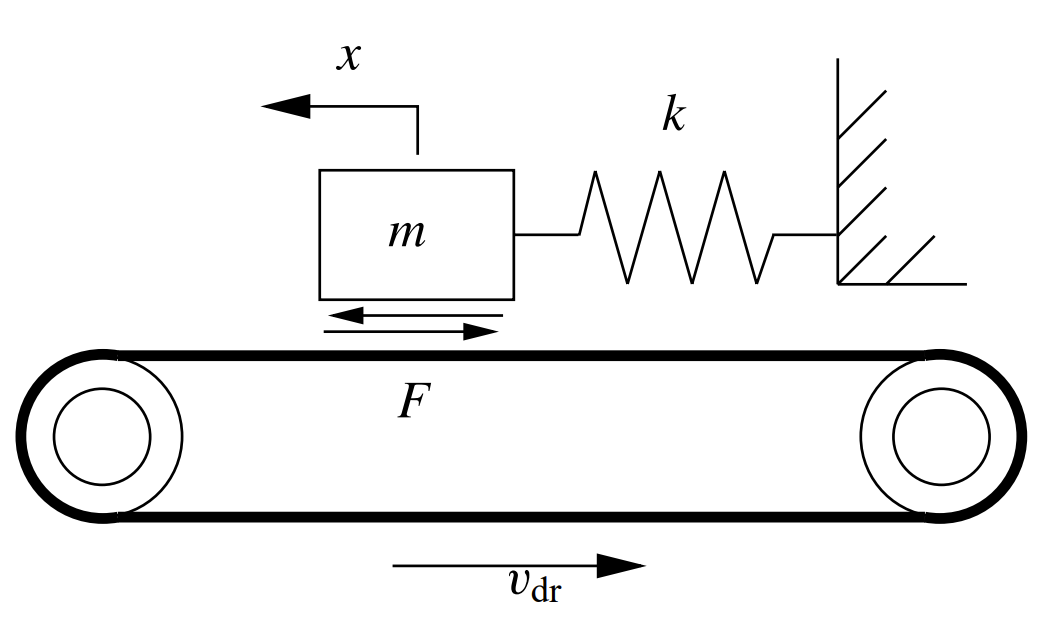
\includegraphics[width=\textwidth]{images/Screenshot_StickSlip.png}
		\caption{System sketch taken from \autocite{leine1998stick}}
	\end{subfigure}
	\hfill
	\begin{subfigure}{0.58\textwidth}
		\centering
		\begin{tabular}{lll}
			\toprule
			Quantity & Symbol & Value \\
			\midrule
			Mass & $m$ & 1 kg \\
			Spring Constant & $k$ & 1 N/m \\
			Belt Velocity & $v_b$ & 0.2 m/s \\
			Max Static Friction Force & $F_s$ & 1 N \\
			Phys. Constant & $\delta$ & 3.0 s/m \\
			\bottomrule
		\end{tabular}
		\caption{Parameters as in \autocite{meyer2020numerical}}
	\end{subfigure}
	\caption{Stick-slip oscillator overview}
	\label{fig:StickSlipOscillator}
\end{figure}

\noindent
\autocite{meyer2020numerical} gives us two switched ODE formulations (one using filippov behavior and one that does not) of second order (order of derivatives present). In each case the state of the system is described by the vector $\mathbf{x}(t)=(x_1(t), x_2(t))^T$, where $x_1$ is the horizontal position of the weight and $x_2$ is the horizontal velocity. From here we get:
\begin{align}
	\dot{\mathbf{x}}(t)= \begin{bmatrix} x_2(t) \\ -\frac{k}{m}x_1(t) + \frac{F(x_1(t), v_{\text{rel}}(t))}{m} \end{bmatrix}
\end{align}
where $v_{\text{rel}}(t) := x_2(t) - v_b$ is the mass' velocity relative to the belt. However, both formulations differ in the way they implement the function $F$. 

\noindent
The non-Filippov version uses
\begin{align}
	F_{\text{nF}}(x_1, \vrel) := \left\{ \begin{matrix}
		min\{ |kx_1|, F_s \} \text{sgn}(kx_1) & \text{if } \vrel = 0 & \text{Stick} \\
		-\frac{F_s\text{sgn}(\vrel)}{1+\delta|\vrel|} & \text{if } \vrel \neq 0 & \text{Slip}
	\end{matrix} \right. \label{eq:F1}
\end{align}
whereas the Filippov version uses
\begin{align}
	F_{\text{F}}(x_1, \vrel) := \left\{ \begin{matrix}
		\frac{-F_s}{1+\delta \vrel} & \text{if } \vrel > 0 & \text{Slip} \\
		\frac{F_s}{1-\delta \vrel} & \text{if } \vrel < 0 & \text{Slip}
	\end{matrix} \right. \label{eq:F2}
\end{align}
The Stick mode in the latter version is expressed as the overlap of both cases (Filippov behaviour).

\subsection{A Connection between the Formulations}
It can easily be checked that \autoref{eq:F1} and \autoref{eq:F2} coincide if $\vrel \neq 0$. The only thing worth explaining is the case $\vrel = 0$ where the mass sticks to the belt. We start by verifying the correctness of the non-Filippov formulation.\\ From here on let $\vrel = 0$.
During the "Stick" phase the mass doesn't experience any acceleration due to the constant motion of the the conveyor belt. Hence, we get that $\dot{x}_2 \overset{!}{=} 0$ during that period of time. From here it follows that
\begin{align*}
	0 \overset{!}{=} \dot{x}_2 = - \frac{k}{m}x_1 + \frac{F_{\text{nF}}(x_1, \vrel)}{m}  \hspace{20pt}
	\Leftrightarrow \hspace{20pt} F_{\text{nF}}(x_1, \vrel) = kx_1
\end{align*}
and as long as $|kx_1| \leq F_s$ we get $$ kx_1 = min\{ |kx_1|, F_s \} \text{sgn}(kx_1) = F_{\text{nF}}(x_1, \vrel) $$ (the first case in \autoref{eq:F1}).
\\ \\
In the Filippov case however, the convex combination parameter $\alpha(t) \in [0, 1]$ is chosen such that $ \alpha \dot{\mathbf{x}}_- + (1-\alpha)\dot{\mathbf{x}}_+ \parallel \vrel = 0 $ (The notation here is as in \autocite{meyer2020numerical}). For the above Stick-Slip-example we can actually write $\alpha$ as an expression of $x_1$.
\begin{lemma} \label{lemma:alpha}
	Let $\dot{\mathbf{x}}$ be the Filippov variant of the above system. Let the rest of the notation be as above with $\vrel=0$ ("Stick"-mode). Then
	\begin{align*}
		\alpha \dot{\mathbf{x}}_- + (1-\alpha)\dot{\mathbf{x}}_+ \parallel \vrel = 0 \hspace{20pt} \text{when} \hspace{20pt} \alpha(t) = \frac{F_s - kx_1(t)}{2F_s}
	\end{align*}
\end{lemma}
\begin{proof}
	First we note that $\dot{\mathbf{x}}_-$ and $\dot{\mathbf{x}}_+$ differ only in their switch in $F_{\text{F}}$. Additionally, the condition $0\overset{!}{=}\vrel=x_2 - v_b$ only places restrictions on $ x_2 $. From this we know that $\vrel=0 \perp (1, 0)^T$. The direction of Filippov sliding must therefore be $a\mathbf{e}_1$ for some $a\neq0$.\\ \\
	To ensure not leaving the switching manifold, $\alpha$ must enforce $ \alpha \dot{x}_2^- + (1-\alpha) \dot{x}_2^+ =0 $. Taking all of this into account, the Filippov-condition reduces to:
	\begin{align*}
		0 &\overset{!}{=} \alpha \dot{x}_2^- + (1-\alpha) \dot{x}_2^+ \\
		&= \alpha \left(-\frac{k}{m}x_1 + \frac{F_{\text{F}}^-(x_1, \vrel)}{m}\right) + (1-\alpha)\left( -\frac{k}{m}x_1 + \frac{F_{\text{F}}^+(x_1, \vrel)}{m} \right) \\
		&= -\frac{k}{m}x_1 + \frac{\alpha F_{\text{F}}^-(x_1, \vrel) + (1-\alpha)F_{\text{F}}^+(x_1, \vrel)}{m}
	\end{align*}
	From this we get:
	\begin{align}
		\alpha F_{\text{F}}^-(x_1, \vrel) + (1-\alpha)F_{\text{F}}^+(x_1, \vrel) \overset{!}{=} kx_1 \label{eq:finalFilCondition}
	\end{align}
	Now for $\vrel=0$:
	\begin{align}
		F_{\text{F}}^-(x_1, \vrel) = \frac{-F_s}{1+\delta \vrel} = -F_s \hspace{20pt} \text{and} \hspace{20pt} F_{\text{F}}^+(x_1, \vrel) = \frac{F_s}{1-\delta \vrel} = F_s \label{eq:FFFFs}
	\end{align}
	Combining \autoref{eq:finalFilCondition} and \autoref{eq:FFFFs}, we can finally solve for $\alpha$:
	\begin{align*}
		\alpha -F_s + (1-\alpha)F_s \overset{!}{=} kx_1 \hspace{20pt} \Leftrightarrow \hspace{20pt} \alpha = \frac{F_s - kx_1}{2F_s}
	\end{align*}
\end{proof}
\begin{remark}
	In \autoref{eq:finalFilCondition} we can see: The general Filippov condition ensures in a somewhat "natural" way, that $\alpha$ must be chosen such that the convex combination of $ F_{\text{F}}^- $ and $F_{\text{F}}^+$ matches the explicit formulation in \autoref{eq:F1} for the "Stick"-mode.
\end{remark}
\begin{remark}
	Again, it needs to be stressed that the expression for $\alpha$ as in \autoref{lemma:alpha} is only analytical in terms of the numerical solution to $x_1(t)$. As of now, we do not have an analytical solution for this expression!
\end{remark}
	
	\newpage
	
	\appendix
	
	\printbibliography
	
\end{document}
